\documentclass[10pt,conference]{IEEEtran}
\IEEEoverridecommandlockouts
\usepackage{cite}
\usepackage{amsmath,amssymb,amsfonts}
\usepackage{graphicx}
\usepackage{booktabs}
\usepackage{url}
\usepackage{textcomp}
\graphicspath{{figures/}}
% Auto-generated by analysis/emit_macros.py. Do not edit.
% Missing computations become \textbf{UNAVAILABLE}, never a guessed number.
\newcommand{\OpenShare}{8.3\%}
\newcommand{\OpenShareFrac}{5932/71677}
\newcommand{\OpenShareCI}{8.1--8.5}
\newcommand{\HeadlineTreatment}{B}
\newcommand{\PrShareA}{77.0\%}
\newcommand{\RepoShareAllA}{40.9\%}
\newcommand{\RepoShareGeTwoA}{71.9\%}
\newcommand{\NPairsA}{1666362}
\newcommand{\NCrossPairsA}{10928}
\newcommand{\PrShareB}{62.4\%}
\newcommand{\RepoShareAllB}{32.6\%}
\newcommand{\RepoShareGeTwoB}{65.6\%}
\newcommand{\NPairsB}{260392}
\newcommand{\NCrossPairsB}{4699}
\newcommand{\PrShareC}{63.2\%}
\newcommand{\RepoShareAllC}{37.4\%}
\newcommand{\RepoShareGeTwoC}{65.8\%}
\newcommand{\NPairsC}{279209}
\newcommand{\NCrossPairsC}{5524}
\newcommand{\NReposIntra}{2156}
\newcommand{\NReposCross}{231}
\newcommand{\NReposMatched}{212}
\newcommand{\NReplayCandidates}{3707}
\newcommand{\LegacyAttempted}{747}
\newcommand{\LegacyEvaluable}{716}
\newcommand{\LegacyIntraRate}{19.8\%}
\newcommand{\LegacyIntraFrac}{119/601}
\newcommand{\LegacyIntraCI}{16.8--23.2}
\newcommand{\LegacyCrossRate}{41.7\%}
\newcommand{\LegacyCrossFrac}{48/115}
\newcommand{\LegacyCrossCI}{33.1--50.9}
\newcommand{\LegacySharedEval}{60}
\newcommand{\LegacyMcNemarP}{$p=0.078$}
\newcommand{\LegacyCrossOnly}{15}
\newcommand{\LegacyIntraOnly}{6}
\newcommand{\LegacyMatchedIntra}{28.3\%}
\newcommand{\LegacyMatchedCross}{43.3\%}
\newcommand{\LegacyExpectedCross}{37.4\%}
\newcommand{\LegacyObservedCross}{41.7\%}
\newcommand{\LegacyFisherP}{$p=0.093$}
\newcommand{\LegacyMultiIntra}{28.6\%}
\newcommand{\LegacySingleIntra}{18.8\%}
\newcommand{\LegacyMultiFrac}{18/63}
\newcommand{\LegacySingleFrac}{101/538}
\newcommand{\LegacyConfPairs}{167}
\newcommand{\LegacyConfFiles}{1646}
\newcommand{\LegacyTypeSignals}{1652}
\newcommand{\LegacySrcFiles}{84.4\%}
\newcommand{\LegacyAddAdd}{15.1\%}
\newcommand{\LegacyModDel}{26.8\%}
\newcommand{\LegacyContent}{57.6\%}
\newcommand{\LegacyStructural}{42.3\%}
\newcommand{\OverlapMeanHours}{41.3}
\newcommand{\OverlapShare1h}{59.0\%}
\newcommand{\OverlapShare24h}{81.1\%}
\newcommand{\CrossPairShare}{1.8\%}
\newcommand{\CrossPairN}{4699}
\newcommand{\CrossPairDenom}{260392}
\newcommand{\AgentIntraClaudeCode}{16.7\%}
\newcommand{\AgentIntraClaudeCodeFrac}{3/18}
\newcommand{\AgentIntraCopilot}{17.8\%}
\newcommand{\AgentIntraCopilotFrac}{38/213}
\newcommand{\AgentIntraCursor}{26.8\%}
\newcommand{\AgentIntraCursorFrac}{11/41}
\newcommand{\AgentIntraDevin}{35.6\%}
\newcommand{\AgentIntraDevinFrac}{31/87}
\newcommand{\AgentIntraOpenAICodex}{14.9\%}
\newcommand{\AgentIntraOpenAICodexFrac}{36/242}
\newcommand{\NPopPRs}{71677}
\newcommand{\NPopRepos}{6673}
\newcommand{\WPThreeStatus}{UNAVAILABLE}
\newcommand{\WPFourStatus}{UNAVAILABLE}
\newcommand{\WPFiveStatus}{UNAVAILABLE}
\newcommand{\WPSixStatus}{UNAVAILABLE}


\begin{document}

\title{Merge Conflicts Among Concurrent Agentic Pull Requests:\\Prevalence, Composition, and a Human Baseline}

\author{
\IEEEauthorblockN{Anonymous Authors}
\IEEEauthorblockA{Paper submitted to SANER 2027, Agentic AI4SE Track. Double-anonymous review.}
}

\maketitle

\begin{abstract}
Concurrent agent-authored pull requests are common, and they conflict at a measurable rate. That rate is not yet known to be higher, lower, or indistinguishable from concurrent human work in the same repositories: the human baseline replay is \WPFourStatus. After excluding the \OpenShareFrac{} pull requests still open at the AIDev-pop cutoff (\OpenShare, Wilson 95\% CI \OpenShareCI), \PrShareB{} of resolved agent PRs overlap another resolved agent PR in the same repository. Treating unresolved PRs as open until cutoff inflates that share to \PrShareA. Cross-agent pairs are \CrossPairShare{} of overlapping pairs (\CrossPairN/\CrossPairDenom) and occur in \NReposCross{} repositories.

A previously drawn earliest-pair \texttt{merge-tree} sample (\LegacyAttempted{} pairs, \LegacyEvaluable{} evaluable) found textual conflict in \LegacyIntraRate{} of intra-agent pairs (\LegacyIntraFrac, CI \LegacyIntraCI) and \LegacyCrossRate{} of cross-agent pairs (\LegacyCrossFrac, CI \LegacyCrossCI). That gap is not a contrast of independent samples. Sixty-four repositories appear in both strata. Within the \LegacySharedEval{} repositories evaluable in both, intra-agent conflict is \LegacyMatchedIntra{} and cross-agent conflict is \LegacyMatchedCross{}; McNemar exact \LegacyMcNemarP{} (\LegacyCrossOnly{} cross-only vs.\ \LegacyIntraOnly{} intra-only discordant pairs). Independent combination of the two agents' intra rates expects \LegacyExpectedCross{} against the observed \LegacyObservedCross. We do not treat the unmatched doubling as a cross-vendor penalty.

The confirmatory design---uniform pair selection, a \NReposMatched-repository match, GEE adjustment, and a same-repo human--human and human--agent replay---is pre-registered. Its conflict rates are \WPThreeStatus{} until those replays finish. Structural signals are \LegacyStructural{} of legacy conflict types.
\end{abstract}

\begin{IEEEkeywords}
merge conflicts, coding agents, pull requests, co-activity, empirical software engineering
\end{IEEEkeywords}

\section{Introduction}
\label{sec:intro}

Coding agents now open pull requests as first-class authors~\cite{li2025aidev,li2026aidevpop}. When two such PRs are open on the same repository, Git sees the same problem it has always seen: concurrent edits that may not merge~\cite{brun2013crystal,sarma2012palantir}. The unit of interest here is \emph{inter-PR} conflict among concurrently open PRs, not the conflict between a single PR and the default branch. AgenticFlict studies the latter at large scale~\cite{ogenrwot2026agenticflict}. We study the former.

A previous draft of this work reported that intra-agent co-active pairs conflicted at \LegacyIntraRate{} and cross-agent pairs at \LegacyCrossRate, and treated non-overlapping Wilson intervals as a finding. That comparison does not survive the committed pair-level file. The two strata share repositories. Agent identity varies by more than the intra/cross gap. Unresolved PRs were treated as open through the end of the observation window, so co-activity was inflated by construction. The earliest overlapping pair in each repository was the only pair replayed.

This paper rebuilds the study around claims that remain after those defects are named. The primary claim is a comparison of agent--agent conflict against a matched human--human baseline in the same repositories, with the same interval logic and the same \texttt{git merge-tree} replay. That comparison is \WPFourStatus{} in this snapshot because human PRs are not in AIDev-pop and GitHub collection has not been run. The secondary claim is already supported by the committed replay file: the unmatched cross-agent gap attenuates under matching and is close to a compositional expectation from agent identity. The tertiary claim is that structural conflict signals (\texttt{modify/delete}, \texttt{add/add}, and related types) are a large share of agent--agent conflict types; whether that share exceeds a human profile is a WP4 test.

We contribute (1)~a censoring-robust measurement of co-activity on a hash-pinned AIDev-pop snapshot, (2)~a pre-registered sampling and testing plan with Holm correction within families~\cite{holm1979}, (3)~a re-analysis of the legacy 747-pair replay that reports the matched McNemar test and the compositional check the earlier draft omitted, and (4)~a replay pipeline whose git flags are pinned so a reviewer can regenerate every number the paper prints.

\section{Background and related work}
\label{sec:related}

\subsection{What we measure}
Brun et al.\ distinguish textual merge conflicts, subsequent build failures, and test failures~\cite{brun2013crystal}. Palant\'ir and Crystal detect the first class early by sharing workspace information or by speculative merges~\cite{sarma2003palantir,sarma2012palantir,brun2011proactive,brun2010speculative}. WeCode similarly moves detection before commit~\cite{guimaraes2012wecode}. This paper measures the textual layer on all sampled pairs. The build and test layers are defined on a scoped subset; they are \WPFiveStatus{} here because Docker is not available in the current environment. We do not describe three layers in the introduction and then measure one.

\subsection{Classic merge-conflict research}
Developers monitor conflicts reactively and judge resolution difficulty from perceived complexity and local expertise~\cite{nelson2019lifecycle,mckee2017perspectives}. Conflict prediction can pre-filter speculative merges~\cite{owhadi2019predicting}. Semi-structured merge changes which textual conflicts appear~\cite{apel2011semistructured,accioly2018semistructured,cavalcanti2017semistructured}. Cassandra schedules tasks to avoid overlapping edits~\cite{kasi2013cassandra}. Our framing is that this literature returns when agents, rather than humans, are the concurrent authors. We therefore cite it, and we do not claim to be the first study of merge conflicts.

\subsection{Agentic pull requests}
Li, Zhang, and Hassan released AIDev and the $>$100-star AIDev-pop subset~\cite{li2025aidev,li2026aidevpop}. AgenticFlict replays agent PRs against a base and reports a 27.67\% conflict rate on a different unit of analysis~\cite{ogenrwot2026agenticflict}. We do not claim the largest empirical study of agentic merge conflicts. We claim the first measurement of \emph{inter-PR} conflict among concurrently open agentic PRs, with a pre-registered human baseline in the same repositories.

\section{Study design}
\label{sec:design}

The analysis plan is committed in the replication package (\texttt{ANALYSIS\_PLAN.md}) with seeds, exclusion rules, covariate lists, and confirmatory tests frozen before any WP3--WP6 model was run. Analyses conceived after that commit are labeled exploratory.

\subsection{Corpus}
We vendor AIDev-pop \texttt{pull\_request.parquet} and \texttt{repository.parquet} from Hugging Face \texttt{hao-li/AIDev}. SHA-256 hashes are in \texttt{data/derived/snapshot.json}. The snapshot contains \NPopPRs{} pull requests in \NPopRepos{} repositories. Agents present in the file are retained, including Google Jules. No agent is dropped silently. Human-authored PRs are not in this table; they require GitHub collection (WP4).

\subsection{Intervals and censoring}
For pull request $i$, $s_i$ is \texttt{created\_at}. The observed resolution time $r_i$ is \texttt{closed\_at} if present, else \texttt{merged\_at}. A PR is censored if both timestamps are null. \OpenShareFrac{} PRs are censored (\OpenShare). End-time treatments: (A)~legacy, $e_i = r_i$ or the snapshot cutoff; (B)~drop censored PRs; (C)~impute $e_i = \min(s_i + m_a, T)$ where $m_a$ is the median resolved lifetime of that agent. Two PRs overlap at slack $k$ iff $\max(s_A,s_B) < \min(e_A,e_B) + k$ days. At $k{=}0$ the overlap must be strictly positive.

The pre-registered headline rule selects B if $|p_A-p_B|\ge 0.05$ or the relative difference is at least 10\%, else A. The data select B. All three treatments appear in Table~\ref{tab:prevalence}.

\subsection{Conflict replay}
A pair is evaluable if \texttt{git merge-tree --write-tree} on the two PR heads exits 0 (CLEAN) or 1 (CONFLICT). Fetch failures, missing merge-bases, timeouts, and other exits are reported as unavailable and never coded as CLEAN. Replay always passes \texttt{-c merge.conflictStyle=merge -c diff.renameLimit=400 -c merge.renames=true}. The recorded git version is in \texttt{data/derived/environment\_record.json}.

\subsection{Sampling}
The legacy sample used \texttt{first\_overlap}: the earliest overlapping pair in each repository, all 122 cross-agent repositories, and a seed-42 draw of 625 intra-agent repositories. That sample is biased toward the start of each repository's agentic history. We keep it as a labeled sensitivity.

The confirmatory design (WP2) uses treatment B at $k{=}0$. Among repositories with at least one intra pair, we draw 625 repositories and one intra pair uniformly. Among repositories with at least one cross pair we take a census of repositories and one cross pair uniformly. For every repository with both kinds of pair (\NReposMatched{} repositories) we draw one intra and one cross pair (designed match). Up to five pairs per stratum per repository are drawn for bootstrap support. This snapshot contains \NReplayCandidates{} unique candidate pairs. Their replay is \WPThreeStatus.

\subsection{Tests}
Wilson score intervals use $z=\Phi^{-1}(0.975)$~\cite{wilson1927}. Comparisons use Fisher exact tests and Newcombe risk-difference intervals~\cite{newcombe1998}, or exact McNemar on matched pairs. Holm correction is applied within each pre-registered family~\cite{holm1979}. We do not treat non-overlapping confidence intervals as a test. The primary confound-controlled test for the cross-agent effect is McNemar on the designed match, not the unmatched 2$\times$2.

\section{RQ1: Co-activity}
\label{sec:rq1}

\begin{table}[t]
\centering
\caption{Co-activity at $k{=}0$ under three end-time treatments. Treatment A treats unresolved PRs as open until the snapshot cutoff. Treatment B drops them. Treatment C imputes the agent-specific median lifetime. Headline treatment is B (pre-registered 5pp/10\% rule).}
\label{tab:prevalence}
\begin{tabular}{l r r r r r}
\hline
T & PRs & PR co-active \% [95\% CI] & Repos w/ pair \% & Pairs & Cross pairs \\
\hline
A & 71,677 & 77.0 [76.7, 77.3] & 40.9 & 1,666,362 & 10,928 \\
B & 65,745 & 62.4 [62.1, 62.8] & 32.6 & 260,392 & 4,699 \\
C & 71,677 & 63.2 [62.9, 63.6] & 37.4 & 279,209 & 5,524 \\
\hline
\end{tabular}
\end{table}



Open PRs are \OpenShare{} of the snapshot. Under treatment A they overlap every later PR in the repository by construction. Table~\ref{tab:prevalence} shows the effect. PR-level co-activity falls from \PrShareA{} to \PrShareB. The 14.6 point drop exceeds the pre-registered threshold, so B is the headline. Treatment C (impute) is close to B (\PrShareC).

\begin{table}[t]
\centering
\caption{Headline treatment B: co-activity versus slack $k$.}
\label{tab:ksweep}
\begin{tabular}{r r r r}
\hline
$k$ (days) & PR co-active \% & Repo co-active \% ($\ge$2 PRs) & Pairs \\
\hline
0 & 62.4 & 65.6 & 260,392 \\
1 & 89.9 & 85.1 & 3,703,720 \\
3 & 91.6 & 87.8 & 8,702,558 \\
7 & 93.0 & 90.3 & 16,810,115 \\
\hline
\end{tabular}
\end{table}



Figure~\ref{fig:censoring} and Figure~\ref{fig:kcurve} show the $k$ sweep. Slack of one day restores most of the PR-level share even under B, because many non-overlapping PRs sit close in time. Overlap duration among B pairs at $k{=}0$ has mean \OverlapMeanHours{} hours; \OverlapShare1h{} last under one hour and \OverlapShare24h{} last under one day. Co-activity is often brief. A binary co-active flag hides that.

\begin{figure}[t]
\centering
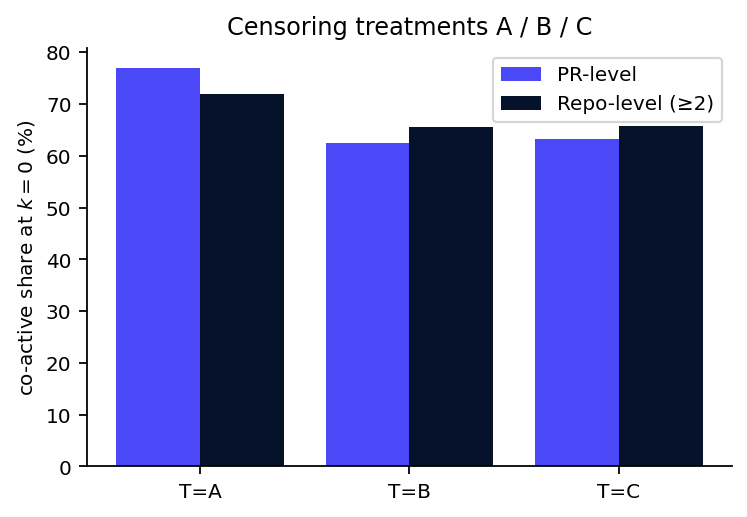
\includegraphics[width=\columnwidth]{fig_censoring.png}
\caption{PR-level and repo-level co-activity at $k{=}0$ under treatments A, B, and C.}
\label{fig:censoring}
\end{figure}

\begin{figure}[t]
\centering
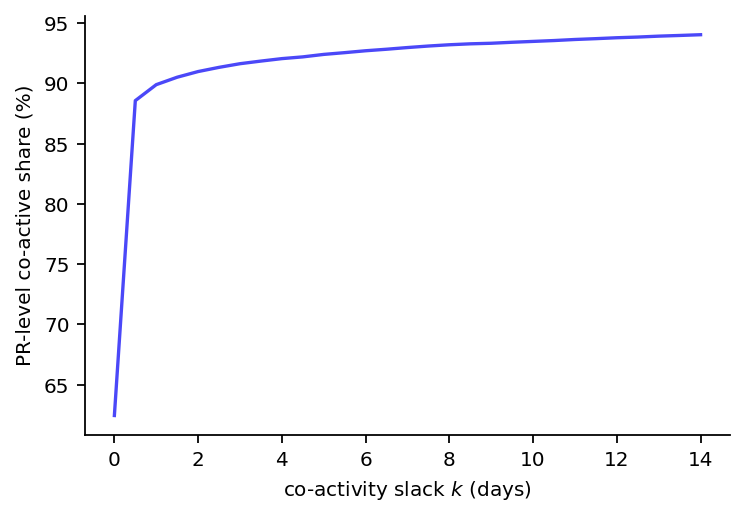
\includegraphics[width=\columnwidth]{fig_kcurve.png}
\caption{PR-level co-activity as a function of slack $k$ under headline treatment B.}
\label{fig:kcurve}
\end{figure}

Cross-agent pairs are rare as a share of pairs (\CrossPairShare) and not rare as a share of repositories that have any pair: \NReposCross{} repositories have at least one cross pair, and \NReposMatched{} of them also have an intra pair. The earlier draft's wording that PRs were co-active ``with another pull request authored by another agent'' is false for this corpus. Almost all co-activity is same-agent.

One repository (\texttt{mochilang/mochi}, Scheme, 13{,}461 agent PRs) dominates pair counts. PR-level rates still count each PR once; pair-level quantities do not. We report both. An exploratory exclusion of repositories with more than 500 PRs is not a confirmatory analysis.

\section{RQ2: Textual conflict rates}
\label{sec:rq2}

\subsection{Legacy earliest-pair sample}
The committed file \texttt{rq3\_merge\_replay\_full.csv} contains \LegacyAttempted{} pairs, of which \LegacyEvaluable{} are evaluable (25 \texttt{UNAVAIL\_fetch}, 6 \texttt{UNAVAIL\_nobase}). Intra-agent conflict is \LegacyIntraFrac{} $=$ \LegacyIntraRate{} (CI \LegacyIntraCI). Cross-agent conflict is \LegacyCrossFrac{} $=$ \LegacyCrossRate{} (CI \LegacyCrossCI). Figure~\ref{fig:legacy} plots those two rates. They are a sensitivity, not the confirmatory estimate.

\begin{figure}[t]
\centering
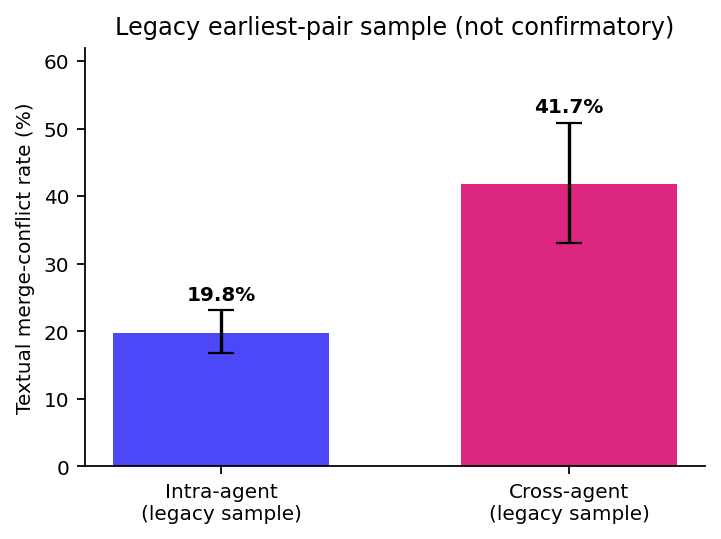
\includegraphics[width=\columnwidth]{fig_legacy_rates.png}
\caption{Legacy earliest-pair sample. Not the confirmatory WP2 sample.}
\label{fig:legacy}
\end{figure}

Realized friction---both PRs merged---is a pre-registered variant. It is not substituted for the primary evaluable rate.

\subsection{Confirmatory sample}
Uniform-within-repository draws are in \texttt{data/samples/}. Replay of \NReplayCandidates{} unique pairs is \WPThreeStatus. Until that file exists, this paper does not print a confirmatory intra-agent or cross-agent rate, and it does not reuse the legacy 19.8\% as if it were the uniform-pair rate.

\section{RQ3: Composition, not a residual cross penalty}
\label{sec:cross}

The unmatched intra/cross comparison uses overlapping samples. Sixty-four repositories appear in both strata of the legacy file; \LegacySharedEval{} are evaluable in both. In that matched slice, intra-agent conflict is \LegacyMatchedIntra{} (17/60) and cross-agent conflict is \LegacyMatchedCross{} (26/60). Discordant pairs: \LegacyCrossOnly{} cross-only-conflict vs.\ \LegacyIntraOnly{} intra-only. McNemar exact \LegacyMcNemarP. The raw 21.9 point gap narrows to 15 points and is not significant at $\alpha=0.05$.

Intra-agent pairs in multi-vendor repositories (a cross pair from the same repo appears in the sample) conflict at \LegacyMultiIntra{} (\LegacyMultiFrac) vs.\ \LegacySingleIntra{} (\LegacySingleFrac) in single-vendor repositories (Fisher exact \LegacyFisherP). Multi-vendor repositories are more conflict-prone before any cross pair is taken as the unit.

Intra-agent rates by agent in the legacy evaluable intra sample: Codex \AgentIntraOpenAICodex{} (\AgentIntraOpenAICodexFrac), Copilot \AgentIntraCopilot{} (\AgentIntraCopilotFrac), Claude Code \AgentIntraClaudeCode{} (\AgentIntraClaudeCodeFrac), Cursor \AgentIntraCursor{} (\AgentIntraCursorFrac), Devin \AgentIntraDevin{} (\AgentIntraDevinFrac). Agent identity spans more than the unmatched intra/cross gap.

A compositional check assigns each cross pair the independent combination $\hat p_a + \hat p_b - \hat p_a\hat p_b$ of the two agents' intra rates. The mean expectation is \LegacyExpectedCross{} against the observed \LegacyObservedCross. The leftover is a few points, not a doubling.

A logistic model with agent-presence indicators is exploratory and collinear with \texttt{cross}: a cross pair mechanically has two agents. That specification is not the source of the abstract sentence. The McNemar result and the 37.4-vs-41.7 comparison do not have that collinearity problem and agree with attenuation.

The confirmatory GEE odds ratio on the designed \NReposMatched-repository match is \WPThreeStatus. The abstract follows the matched McNemar, not the unmatched 2.9 odds ratio from an unadjusted 2$\times$2.

\section{RQ4: Conflict types}
\label{sec:types}

Among \LegacyConfPairs{} conflicting legacy pairs there are \LegacyConfFiles{} conflicted files and \LegacyTypeSignals{} merge-tree type signals. Content is \LegacyContent. Structural signals are \LegacyStructural{} (\texttt{modify/delete} \LegacyModDel, \texttt{add/add} \LegacyAddAdd, plus rename/delete and file-location). Source-code files are \LegacySrcFiles{} of conflicted paths.

Whether this structural share exceeds a human--human profile in the same repositories is a Family~3 test. It is \WPFourStatus. We do not quote a literature human profile as a substitute.

\section{Human baseline and build/test layers}
\label{sec:wp45}

WP4 collects human PRs in the same repositories and window, classifies authors against the AIDev agent-login set, enumerates human--human and human--agent overlaps with the same interval treatment, and replays them with the same merge-tree wrapper. Status: \WPFourStatus. No literature conflict rate is used as a stand-in.

WP5 materializes textually CLEAN merges in a container for Python, JavaScript/TypeScript, and Go repositories with a detected manifest, with a 15-minute cap, and with timeouts and environment failures coded as their own labels. Status: \WPFiveStatus. We do not call the textual rate a conservative lower bound without this measurement.

\section{Threats to validity}
\label{sec:threats}

\textit{Construct.} Textual \texttt{merge-tree} conflict is not semantic conflict. WP5 is the partial remedy and is not run here.

\textit{Internal.} The legacy sample's earliest-pair rule, the accidental 64-repository stratum overlap, and the collinearity of agent-presence indicators with \texttt{cross} are named because they are in the committed code and CSV. Treatment A inflates co-activity; we therefore headline B. The confirmatory replay is not in this snapshot, so we do not smuggle legacy rates into the confirmatory slot.

\textit{External.} AIDev-pop is repositories with more than 100 stars. One repository contributes 13k agent PRs. PR refs disappear; 25 of 747 legacy pairs were already unfetchable. GitHub collection for humans needs a token and will drift.

\textit{Conclusion.} The unmatched cross-agent gap had low power once matched ($n=60$ pairs of pairs). The designed match has \NReposMatched{} repositories, which is better, and still limited by discordant-pair count. A non-significant McNemar is reported with its discordant split and interval, not as proof of a zero effect.

\section{Conclusion}
\label{sec:conc}

Concurrent agentic PRs are common once censoring is handled honestly: \PrShareB{} of resolved agent PRs overlap another resolved agent PR at $k{=}0$. The unmatched cross-agent doubling in the legacy sample does not survive matching or a compositional check. Structural conflict signals are \LegacyStructural{} of legacy type signals. The question that would make this a comparison rather than a prevalence study---whether agents conflict more than humans on the same repositories---is pre-registered and currently \WPFourStatus. If that comparison lands near equality, the publishable claim is volume plus structure, not a cross-vendor penalty. That is the paper we will write.

An anonymized replication package accompanies the submission. A DOI is restored at camera-ready. \texttt{make all} regenerates every table and figure the paper cites from the committed snapshot, without live GitHub, and prints UNAVAILABLE where a live step has not been run.

\bibliographystyle{IEEEtran}
\bibliography{references}

\end{document}
